\begin{lstlisting}[language=LaTeX, caption=Combination of Side-by-Side and End-by-End Charts Example, label=listing:combination-of-side-by-side-and-end-by-end-charts-example]
\sidebyside[float=!htb]{0.52\linewidth}{
    \begin{BiliFigure}[float=H,label=figure:combination-of-side-by-side-and-end-by-end-charts-example-1]{Perfect Sampling of a Normally Consolidated Clay and an Over-consolidated Clay}{正常固结土和超固结土的完美采样}
        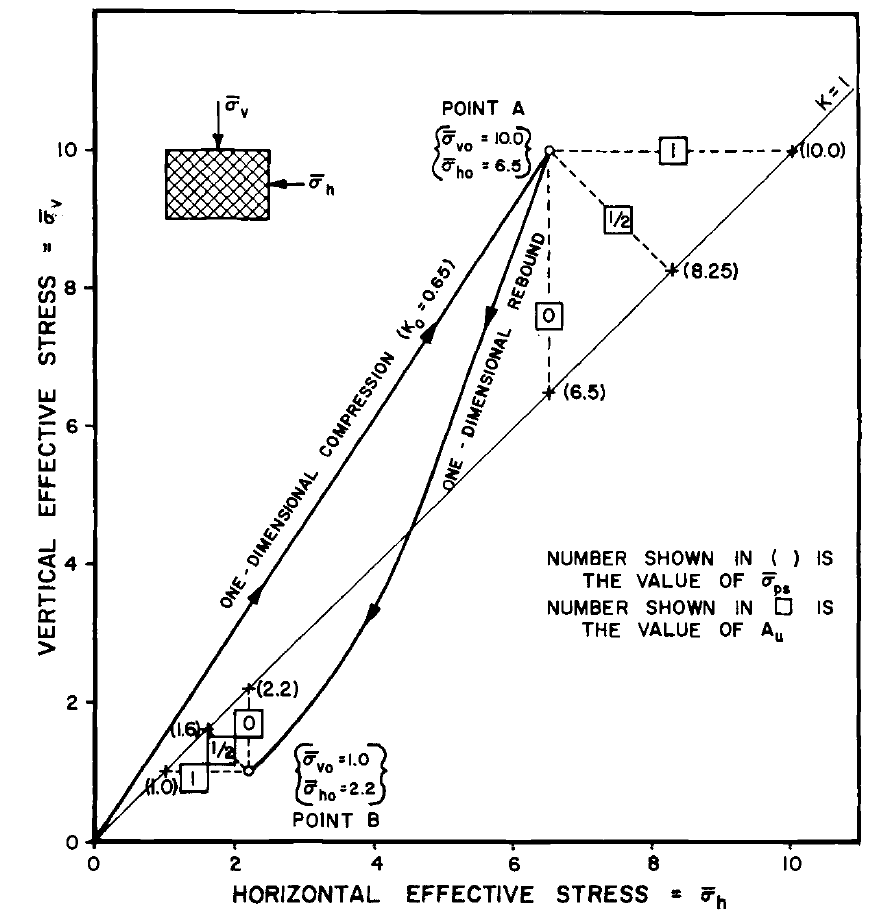
\includegraphics[width=\linewidth]{figures/figure-7.png}
    \end{BiliFigure}
}{0.44\linewidth}{
    \endbyend[float=H]{\linewidth}{
        \begin{BiliFigure}[float=H,label=figure:combination-of-side-by-side-and-end-by-end-charts-example-2]{An example of shear wave velocity measurement}{剪切波速度测量示例}
            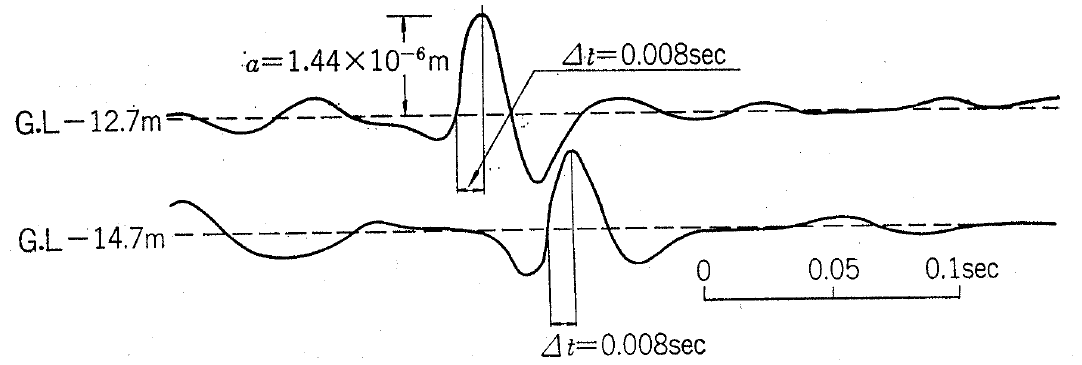
\includegraphics[width=\linewidth]{figures/figure-5.png}
        \end{BiliFigure}
    }{
        \begin{BiliFigure}[float=H,label=figure:combination-of-side-by-side-and-end-by-end-charts-example-3]{Conceptual field loading condition}{概念性的场地加载条件}
            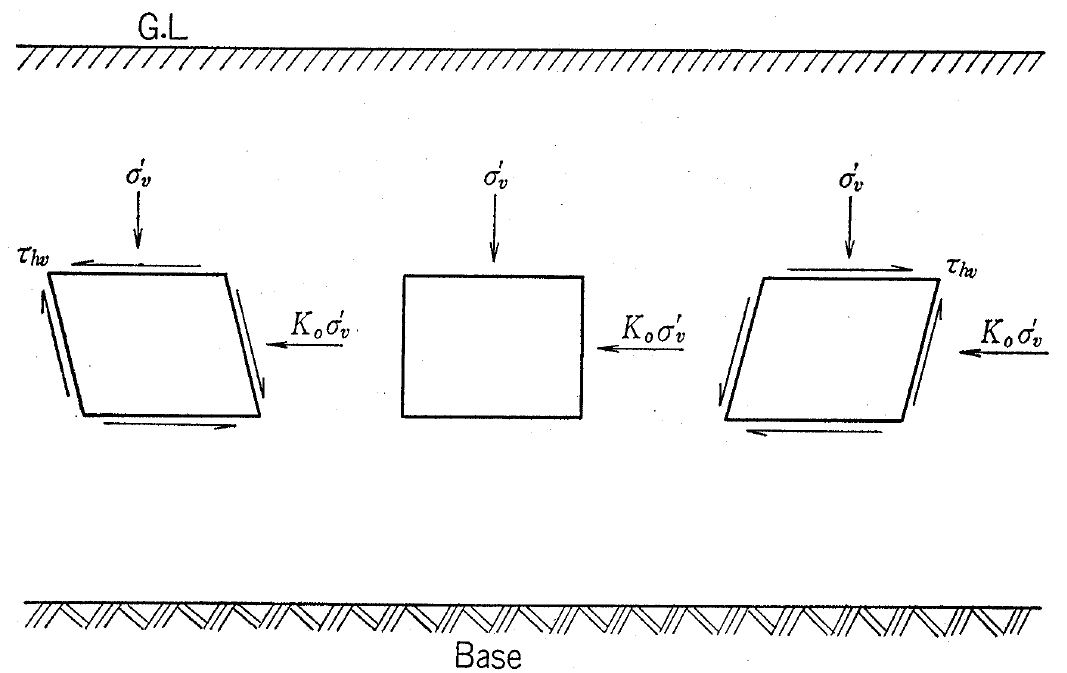
\includegraphics[width=\linewidth]{figures/figure-6.png}
        \end{BiliFigure}
    }
}
\end{lstlisting}

\sidebyside[float=!htb]{0.52\linewidth}{
    \begin{BiliFigure}[float=H,label=figure:combination-of-side-by-side-and-end-by-end-charts-example-1]{Perfect Sampling of a Normally Consolidated Clay and an Over-consolidated Clay}{正常固结土和超固结土的完美采样}
        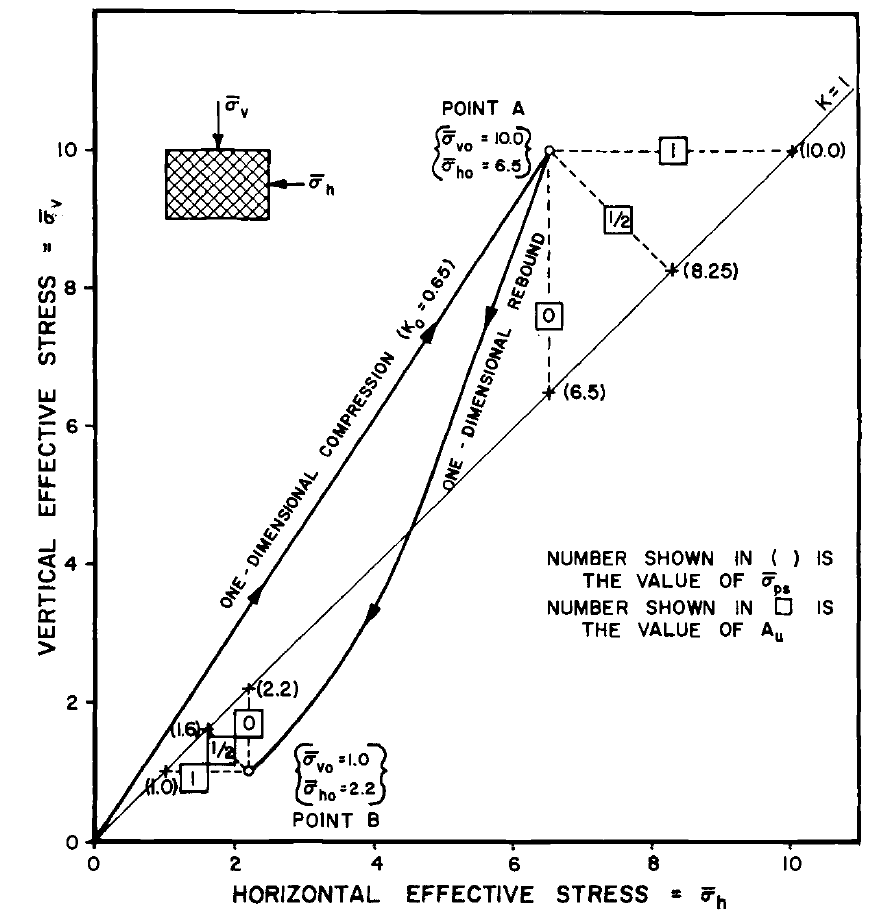
\includegraphics[width=\linewidth]{figures/figure-7.png}
    \end{BiliFigure}
}{0.44\linewidth}{
    \endbyend[float=H]{\linewidth}{
        \begin{BiliFigure}[float=H,label=figure:combination-of-side-by-side-and-end-by-end-charts-example-2]{An example of shear wave velocity measurement}{剪切波速度测量示例}
            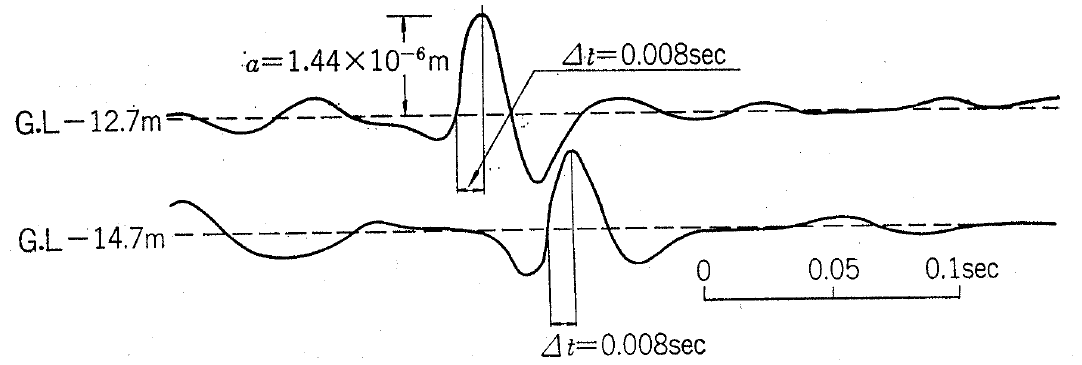
\includegraphics[width=\linewidth]{figures/figure-5.png}
        \end{BiliFigure}
    }{
        \begin{BiliFigure}[float=H,label=figure:combination-of-side-by-side-and-end-by-end-charts-example-3]{Conceptual field loading condition}{概念性的场地加载条件}
            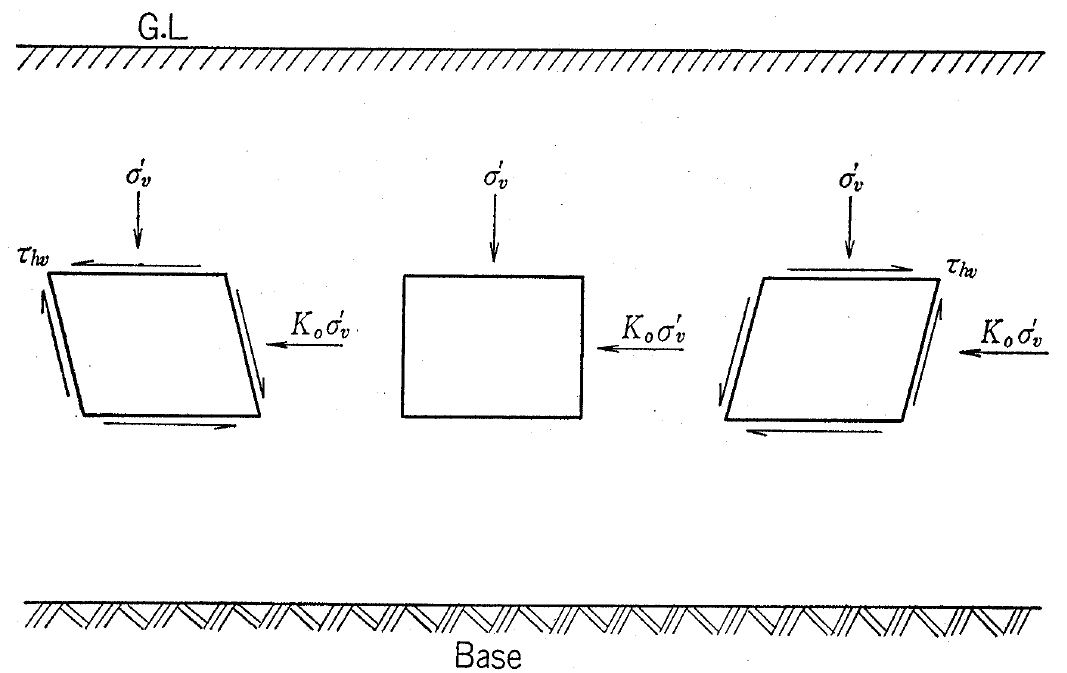
\includegraphics[width=\linewidth]{figures/figure-6.png}
        \end{BiliFigure}
    }
}
